\section{Wnioski i kierunki rozwoju}
\begin{frame}
\frametitle{\secname}

\begin{itemize}
	\item Prosty reaktywny zestaw reguł oparty na \textit{zjawisku respektu} sprawdza się w zatłoczonym środowisku, w którym bieżąca sytuacja zmienia się w sposób bardzo dynamiczny. 
	
	\item Wymuszenie ustępowania pierwszeństwa w oparciu o zasadę \textit{priorytetyzowania wychodzących} w wąskich przejściach zwiększa jego przepustowość. 
	
	\item \textit{Zasada prawej dłoni} nie radzi sobie dobrze przy ograniczonej ilości przestrzeni np. w \textit{wąskich korytarzach}.
	
	\item W bardziej skomplikowanych środowiskach, takich jak na przykład \textit{wąski korytarz} napotykamy na problem ,,przepychania'' się robotów.
	
\end{itemize}

\note{
		
\begin{itemize}
	\item Bazując wyłącznie na zdefiniowanych regułach behawioralnych oraz zasadzie pierwszeństwa jesteśmy w stanie zarządzać grupą robotów w mniej lub bardziej skomplikowanych środowiskach.
	
	\item Przykładem takim może być \textit{zasada prawej dłoni} bazująca na ustępowaniu pierwszeństwa jadącym z prawej strony i dobrze sprawdzająca się na skrzyżowaniach.  Metoda nie radzi sobie najlepiej przy ograniczonej ilości przestrzeni. W takiej sytuacji konieczne jest stosowanie innych metod zarządzania grupą robotów na przykład bazujących na zjawisku respektu.  Nie wszystkie wzorce zachowań dają dobre rezultaty w każdej sytuacji.
	
	\item  W środowiskach bardziej skomplikowanych, jak  \textit{przejście przez drzwi}, lepiej radzą sobie metody, które wymuszają przepustowość traktu komunikacyjnego.  Podnosząc priorytet robotom, które wychodzą z pomieszczenia udrażniamy przejście i tym samym zwiększamy jego przepustowość. 
	
	\item W bardzie skąplikowanych środowiskach koniecznej jest poszukiwanie innych metod koordynacji ruchu robotów.
	
\end{itemize}	
}
\end{frame}
	


\section*{Wnioski i kierunki rozwoju}
\begin{frame}
\frametitle{\secname}

\begin{center}
	\textbf{Możliwe jest stworzenie zdecentralizowanego behawioralnego algorytmu sterowania ruchem robotów opartego na zachowaniu, inspirowanego postępowaniem przemieszczających się osób.}
\end{center}

\note{
	
Analizując poszczególne eksperymenty można stwierdzić, iż postawiona teza pracy została udowodniona. Możliwe jest stworzenie zdecentralizowanego behawioralnego algorytmu sterowania ruchem robotów opartego na zachowaniu, inspirowanego postępowaniem przemieszczających się osób. Rozwiązanie to sprawdza się w środowiskach, w których konieczne jest skuteczne koordynowanie grupą robotów działających w dynamicznie zmieniającym się środowisku.
}
\end{frame}

\section*{Wnioski i kierunki rozwoju}
\begin{frame}
\frametitle{\secname}
\framesubtitle{Hybrydowy algorytm koordynacji ruchu robotów}

\begin{figure}[!hbp]
	\centering
	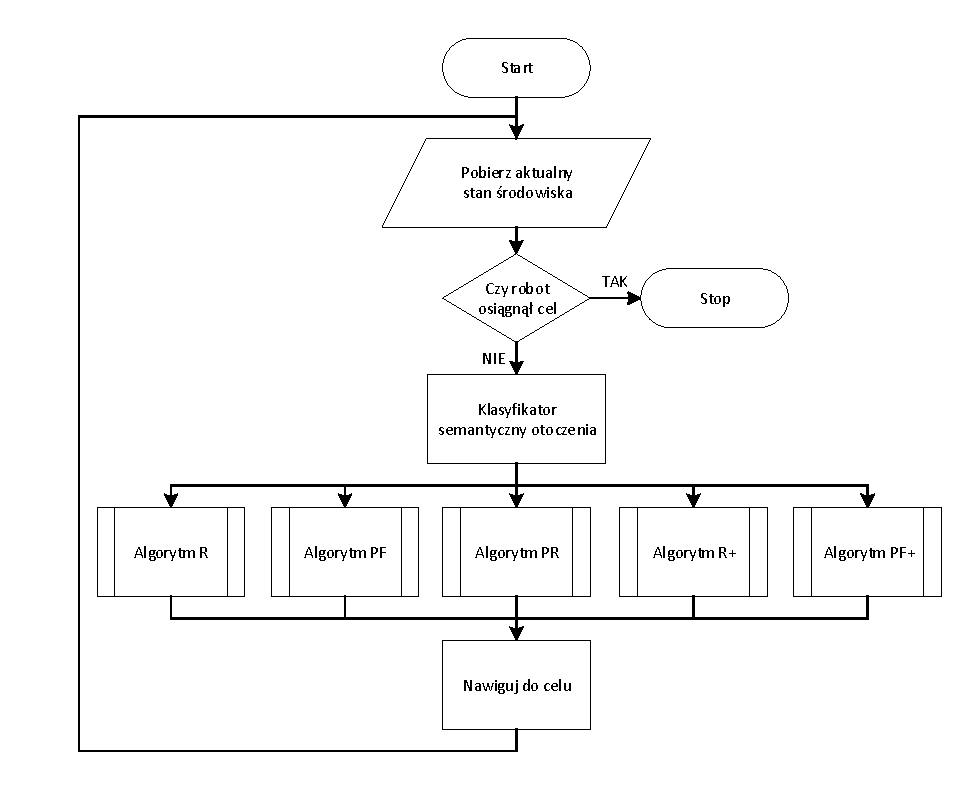
\includegraphics[page=1,width=0.85\textwidth]{img/hybrid_algorithm.pdf}
	
\end{figure} 
\note{
Oczywiście nie każda z metod jest na tyle uniwersalna, że można ją stosować we wszystkich przypadkach. Konieczne jest zatem dobieranie do danej sytuacji metod ją rozwiązujących. 

Połączenie kilku algorytmów, w jedno spójne rozwiązanie, umożliwi dostosowanie rozwiązania w zależności od bieżącej sytuacji. Taka zintegrowana metoda hybrydowa koordynacji ruchu pozwoli na optymalizację działania robota dla konkretnego przypadku. 

}
\end{frame}

\begin{frame}

\begin{center}
	Dziękuje za uwagę
\end{center}

\end{frame}